The asymptotic generalization performance of a learner is of utmost importance since practical machine learning is bound to a finite setting. A learning curve shows the generalization performance of a learner concerning training set size. Learning curves have numerous applications in machine learning pipelines (decrease data collection cost, model selection, hyperparameter tuning, etc.). The training set size creates an evident bottleneck since the computational effort that goes into training increases with the training set size. (Although, numerous methods try to circumvent that bottleneck both for shallow and deep machine learning models \cite{ma2017,kiefer1952}.) This computational bottleneck prevents a reliable learning curve generation. Thus, the need for interpolation and extrapolation of these curves gains importance.

\begin{wrapfigure}{r}{0.5\textwidth}
  \begin{center}
    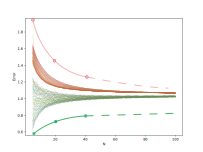
\includegraphics[width=0.5\textwidth]{lc_extrapolate}
  \end{center}
  \caption{Learning curve extrapolation visualization for both training and test performance  with an error measure concerning the training set size $N$.}
\end{wrapfigure}

Historically learning curves are mostly modeled by parametric models, namely exponential, power law, etc.,  to extrapolate the generalization performance concerning training set size. (See \cite{mohr} for detailed references to these parametric methods.) However, for all of these parametric models, there exists an intrinsic monotonicity assumption. As shown in the detailed survey \cite{looga}, expecting a learner to have a monotone generalization error decrease with increased training set size is not reasonable for a given dataset. This is why we propose a data-driven approach for learning curve extrapolation, hoping that will allow us to break free from the monotonicity assumptions stemming from parametric models. 

Fortunately, extensive learning curve databases are getting publicly available which facilitates a data-driven approach to extrapolating learning curves. A data-driven modeling approach to learning curves requires the treatment of learning curve creation as a learning problem in itself. To be precise we will consider a setting where there are available full learning curves from different learners on different datasets, different learners from the same dataset, and a learner for the same dataset with changing hyper-parameters. In addition to full learning curves, we are given a few data points (here few data points refer to \textit{error measure-training set size} pairs). The aim will be to extrapolate this curve to increased training set sizes given the generalization performance of the smaller training set sizes of a learner. 

This paper utilizes functional analysis to extract valuable meta-information that is coming from a database of learning curves via Functional Principal Component Analysis (FPCA) and linearly combines these components while minimizing the squared loss over the observed data points. 


%\subsection{Outline}
%This paper starts with the introduction of the semi-parametric kernel ridge method. Afterward, Section \ref{section:fpca} establishes the background for functional analysis. Then, in Section \ref{section: problem} problem setting is described and the results are presented in Section \ref{section: results}
%





